% Vector posición: base en el origen vs base en P (libro fig. 3.1)
\documentclass[border=5pt]{standalone}
\usepackage{tikz}
\usetikzlibrary{arrows.meta, calc}
\begin{document}
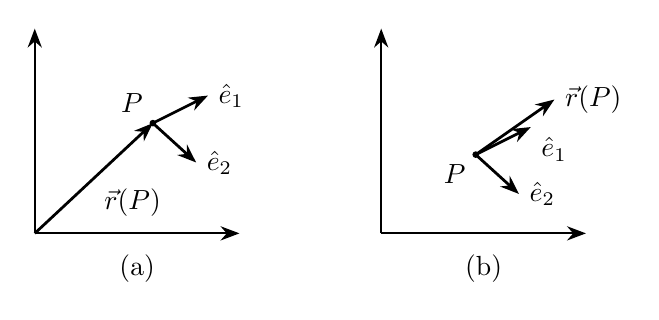
\begin{tikzpicture}[>={Stealth[length=2.4mm]}, line width=0.7pt]
  % --- panel (a): vector desde el origen, base en P ---
  \begin{scope}
    \draw[->] (0,0)--(0,2.6); \draw[->] (0,0)--(2.6,0);
    \coordinate (P) at (1.5,1.4);
    \draw[->, line width=1pt] (0,0)--(P) node[midway,below right]{$\vec r(P)$};
    \fill (P) circle (1.2pt) node[above left]{$P$};
    \draw[->, line width=1pt] (P)--($(P)+(0.7,0.35)$) node[right]{$\hat e_1$};
    \draw[->, line width=1pt] (P)--($(P)+(0.55,-0.5)$) node[right]{$\hat e_2$};
    \node at (1.3,-0.45){(a)};
  \end{scope}
  % --- panel (b): vector y base, ambos desde P ---
  \begin{scope}[xshift=4.4cm]
    \draw[->] (0,0)--(0,2.6); \draw[->] (0,0)--(2.6,0);
    \coordinate (P) at (1.2,1.0);
    \fill (P) circle (1.2pt) node[below left]{$P$};
    \draw[->, line width=1pt] (P)--($(P)+(1.0,0.7)$) node[right]{$\vec r(P)$};
    \draw[->, line width=1pt] (P)--($(P)+(0.7,0.35)$) node[below right]{$\hat e_1$};
    \draw[->, line width=1pt] (P)--($(P)+(0.55,-0.5)$) node[right]{$\hat e_2$};
    \node at (1.3,-0.45){(b)};
  \end{scope}
\end{tikzpicture}
\end{document}
